\chapter{Filtry}
\label{sec:Filters}
\vspace{-30pt}
\

Filtrování signálu je použito pro odstraněni sumu. To je potřeba pro lepší detekce 
fáze auta. Tato sekce popisuje různé filtry typu dolní propust a jejich porovnání.

\section{FIR filtry}\

\textbf{FIR filtry} jsou filtry s koneční impulzní odezvou. Tyto filtry používají jen
hodnoty ze vstupního signálu\cite{FIR}.

\subsection{Klouzavý průměr}\

\textbf{Klouzavý průměr} zprůměruje určitý počet hodnot ze vstupního signálu. 
Ve tvaru rovnice to~bude:
\begin{equation}
y[i] = \frac{1}{M}\sum_{j = 0}^{M - 1}x[i+j],
\end{equation}
kde $y[\,\,]$ je výstupní hodnota, $M$ je počet hodnot a $x[\,\,]$ je vstupní hodnota
\cite{Filters}.

Implementace tohoto filtru byla zjednodušena tím, že když hodnota součtu vstupních 
hodnot se uloží, a zároveň počet hodnot bude se rovnat $M$, přidáním nové hodnoty 
se odečte vstupní hodnota prvního vzorku ze součtu a přičte se hodnota nového. 
Výsledná hodnota se pak vydělí hodnotou~$M$\cite{krokomer}.

Při filtrování signálu byla po experimentech zvolena hodnota M = 8.

\section{IIR filtry}\

\textbf{IIR filtry} jsou filtry s nekoneční impulzní odezvou. Tyto filtry, na rozdíl 
od FIR filtrů, používají mechanizmus zpětné vazby, tzn. výstupní hodnoty\cite{IIR}.

Všichni implementované IIR filtry jsou ve tvaru:
\begin{equation}
y[n] = \sum_{i = 0}^{j}a_{i}x[n - i] + \sum_{i = 1}^{k}b_{i}y[n - i],
\end{equation}
kde $y[\,\,]$ je výstupní hodnota, $x[\,\,]$ je vstupní hodnota a $a_i$ i $b_i$ 
jsou koeficienty.

\subsection{Jednopólová dolní propust}\

Filtr má jen dva koeficienty:
\begin{align}
a_0 &= 1 - x \\
b_1 &= x
\end{align}
kde $x$ je hodnota v intervalu <0;1>, která kontroluje silu filtru\cite{Filters}.

Zvolená hodnota $x$ je 0,85. Z toho plynou hodnoty koeficientu $a_0 = 0,15$ a 
$b_1 = 0,85$.

\subsection{Čtyřstupňová dolní propust}\

Filtr má 5 koeficientu:
\begin{align}
a_0 &= (1 - x)^4 \\
b_1 &= 4x \\
b_2 &= -6x^2 \\
b_3 &= 4x^3 \\
b_4 &= -x^4
\end{align}
kde $x$ je hodnota v intervalu <0;1>, která kontroluje silu filtru\cite{Filters}.

Zvolená hodnota $x$ je 0,6.

\subsection{Dvoupólový Čebyševův filtr}\

Filtr má 5 koeficientu. Tyto koeficienty jsou z tabulky hodnot pro Dvoupólový Čebyševův filtr pro frekvence $f_c = 0,075$ \cite{Filters}:
\begin{align}
a_0 &= 3.869430E-02f \\
a_1 &= 7.738860E-02f \\
a_2 &= 3.869430E-02f \\
b_1 &= 1.392667E+00f \\
b_2 &= -5.474446E-01 \\
\end{align}

\section{Testování}\

Všichni filtry byly testovány pomocí algoritmu řízení po draze, který byl popsán
v kapitole \ref{sec:PlatformControl}. Obrázky \ref{fig:NoFilter} a \ref{fig:filters} 
zobrazují původní nefiltrovány signál a výstupy jednotlivých filtrů 
aplikovaných na tento signál.

\begin{figure}[!h]
	\centering
	\vspace{-5pt}
    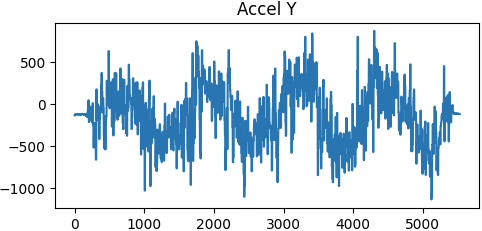
\includegraphics[width = 0.7\linewidth]{Figures/NoFilter.png}
    \caption{Nefiltrovaný signál.}
    \label{fig:NoFilter}
    \vspace{-10pt}
\end{figure}

\begin{figure}[!h]
    \centering
        \subfloat[Klouzavý průměr]{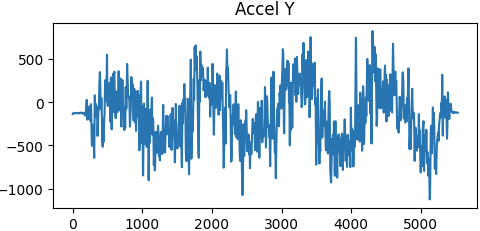
\includegraphics[width = .5\textwidth]{Figures/MovingAverage.png}\label{fig:MovingAverage}}
    \subfloat[Jednopólová dolní propust]{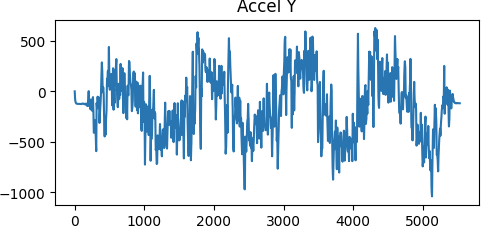
\includegraphics[width = .5\textwidth]{Figures/SinglePole.png}\label{fig:SinglePole}} \\
        \subfloat[Čtyřstupňová dolní propust]{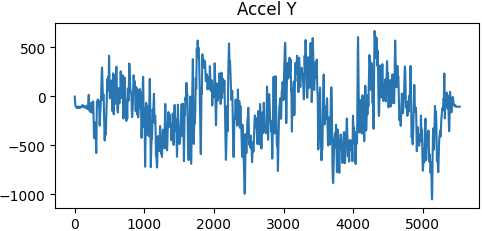
\includegraphics[width = .5\textwidth]{Figures/FourStage.png}\label{fig:FourStage}}
    \subfloat[Dvoupólový Čebyševův filtr]{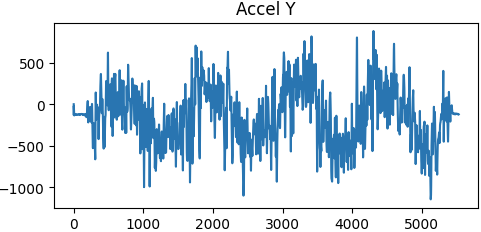
\includegraphics[width = .5\textwidth]{Figures/Chebyshev.png}\label{fig:Chebyshev}}
    \caption{Ukázky aplikovaných filtrů.}
    \label{fig:filters}
\end{figure}

Po porovnání nejlepší výsledky ukázali filtry jednopólová dolní propust a 
dvoupólový Čebyševův filtr. Poslední byl použit pro implementaci, 
protože zachovává amplitudu signálu.
\endinput
